\section{Hierarchical view matching based on Clustering}\label{section:hierarchical}

The first place recognition method presented in this work found inspiration in the human memory of places. Unlike the further proposed methods, this approach does not try to model the brain's other biological structures but tries to conceive biological inspiration more abstractly. The idea is based on the way how humans usually remember places. According to the \cite{memoryHier}, the long-term human spatial memory recall is built upon a hierarchical structure. First, people remember the general layout of the view. Afterward, they can recall basic information about the scene's largest or most significant features, followed by a few more detailed features. Finally, the small details are usually wholly forgotten or recalled at last.\par
The template representation is used based on this behavior. The scene is decomposed into a set of objects based on their location, connection, and color. Each object is simplified as a list of its most significant features, namely the position of its center point, volume and area of its convex hull, and its most significant color. Together with this information, the number of points from the colored point cloud in this object is stored. Afterward, the small, insignificant objects are entirely ignored.\par
During the matching process, the scenes are compared according to these objects. Objects are paired by their similarities based on their stored properties' similarities. The final similarity is calculated as a weighted average of these similarities by the number of points connected with the object. In this way, the largest, usually most significant objects influence the result more than the smaller details.\par

TODO images of an example - scene/representation

\subsection{Template extraction}

The decomposition of the colored point cloud into the set of objects description is a two-step process. In the first step, the scene is decomposed into clusters, representing individual objects. Afterward, in the second step, all clusters are processed independently, and the objects' information is extracted.\par
The clustering is performed using the DBScan algorithm \cite{dbScan} in a six-dimensional space. The first three dimensions standardly represent the points' x, y, and z positions. The additional three dimensions represent points' colors, namely the red, green, and blue components. The standard DBScan algorithm assumes that all dimensions are in the same units. Because there is obviously no standard conversion between color and distance, the color dimensions must be scaled by a suitable scaling factor. The best coefficient has been found experimentally, as well as the DBScan parameters.\par

TODO image of scene before and after the clustering

After the scene is decomposed, each cluster is processed independently of the others. Before the information about the object is extracted,  its convex hull is found using the quick-hull algorithm \cite{quickhull}. After the convex hull is known, its center, volume, and area can be easily calculated. Together with the information obtained from the convex hull, the information about the object's color is extracted. Based on the properties of the DBScan algorithm, it can be expected that all points from the cluster have a similar color. Therefore, storing average color instead of all individual colors leads to negligible information loss. The average color is calculated as an arithmetic average of the red, green, and blue parts of the colors of individual points in the cluster. After calculating, the average color is converted into the chosen color format. The last stored information about the object is the cluster size\footnote{Number of points in the cluster}.\par
All clusters with a size smaller than the given threshold are considered small insignificant objects and are ignored even before the object information extraction process starts.

TODO diagram of the whole process

\subsection{Template matching}

Before calculating the similarity between two whole scenes, we need to describe an approach for comparison of two objects based only on the object properties. We compare four essential properties of the objects: distance between objects, the difference between colors, sizes, and shapes of the objects. The distance of the objects is calculated as the euclidean distance of their centers. The formulas described in section \ref{section:colorModels} are used for the color differences. The size difference is calculated as a difference between the volume of the convex hulls of the objects. For the determination and comparison of the exact shapes, we do not have enough information. However, much information about the shape of many objects is encoded in a ratio between their volume and area. There are, of course, objects with entirely different ratios between volume and area, but for most pairs with different shapes, the ratio between volume and area is also different. So the difference between shapes is represented as a difference in the ratio of volume and area of the convex hulls of the objects.\par
At this point, the absolute difference between objects is known for each essential property, and we have to decide if they are similar enough or not. Therefore the function is needed for each property that takes the property difference as an input and returns a number between 0 and 1, representing the similarity of the individual property. In this work, we choose
$$
    f_{a,x_0}(x) = 1 - \frac{1}{1 + e^{-a(x-x_0)}}
$$
as the wanted function for each property, where $x$ is the input, and $a$ and $x_0$ are parameters specific for each property. This function, illustrated in Figure \ref{fig:sigmoid}, has a property that for differences smaller than the threshold, it is very close to one, for differences larger than the threshold, it is close to 0, and for inputs in the neighborhood of the threshold, it is gradually decreasing. The way how to find the suitable parameters is described in the following section.\par

\begin{figure}[htpb]
    \centering
    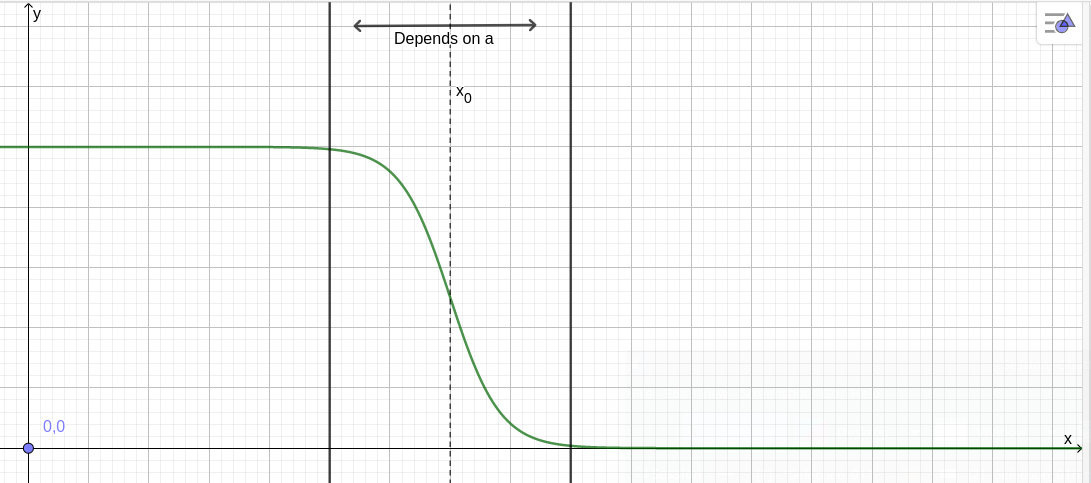
\includegraphics[width=0.8\textwidth]{sigmoid.png}
    \caption{Parametrized sigmoid function} \label{fig:sigmoid}
\end{figure}

After the similarity of each property is calculated, the final similarity of the objects is calculated as a weighted average of the similarities of the individual properties. The weights are found automatically, as described in the following section. The object matching process is summarized in Algorithm \ref{alg:objectSimilarityCalc}.

\begin{algorithm}
    \caption{Objects comparsion}\label{alg:objectSimilarityCalc}
    \begin{algorithmic}
        \Require Objects $O_1$ and $O_2$
        \Ensure Similarity of the objets
        \State $x_1 \leftarrow $ difference in colors between $O_1$ and $O_2$
        \State $x_2 \leftarrow $ difference in positions between $O_1$ and $O_2$
        \State $x_3 \leftarrow $ difference in volume between $O_1$ and $O_2$
        \State $x_4 \leftarrow $ difference in volume/area ration between $O_1$ and $O_2$
        \State $s_1 \leftarrow f_{a_1,x_{0,1}}(x_1)$
        \State $s_2 \leftarrow f_{a_2,x_{0,2}}(x_2)$
        \State $s_3 \leftarrow f_{a_3,x_{0,3}}(x_3)$
        \State $s_4 \leftarrow f_{a_4,x_{0,4}}(x_4)$
        \State $res \leftarrow\frac{w_1s_1 + w_2s_2 + w_3s_3 + w_4s_4}{w_1+w_2+w_3+w_4}$
        \State\Return $res$
    \end{algorithmic}
\end{algorithm}

The method for comparison of the two scenes uses the above-described approach for comparison of the individual objects. First, let's define a scene as an unordered set of objects. Then, let's define the primary scene as the current scene received from the sensors and the secondary scene as the scene from the storage. This approach iterates through all objects in the primary scene and, for each object, calculates the similarities with all objects in the secondary scene. Afterward, for each object in the primary scene, the most similar object from the secondary scene is picked\footnote{Two objects in the primary scene may have the same most similar object from the secondary scene}. Finally, the similarities with the most similar objects are used to calculate the average, weighted by the sizes of the clusters. The whole process is summarized in the Algorithm \ref{alg:scenesSimilarityCalc}.

\begin{algorithm}
    \caption{Scenes comparsion}\label{alg:scenesSimilarityCalc}
    \begin{algorithmic}
        \Require Primary scene $S_1$ and secondary scene $S_2$
        \Ensure Similarity of the scenes
        \State $res := 0$
        \State $sizesTotal := 0$
        \For{$o_1 \in S_1$}
        \State $best := 0$
        \For{$o_2 \in S_2$}
        \State $best \leftarrow \max(best,\text{ CompareObjects($o_1,o_2$)})$
        \EndFor
        \State $res \leftarrow left + best \cdot \text{clusterSize($o_1$)}$
        \State $sizesTotal \leftarrow sizesTotal + \text{clusterSize($o_1$)}$
        \EndFor
        \State $res \leftarrow \frac{res}{sizesTotal}$
        \State\Return $res$
    \end{algorithmic}
\end{algorithm}

\subsection{Automatic parameter tuning}\label{section:parameterTuning}

To make the templates comparison algorithm work, 13 different parameters must be correctly set. Namely, $a$ and $x_0$ parameters for the sigmoid functions for each of four property differences, the weight of each property, and the final threshold. There are naturally many combinations, and every change may strongly influence the results and the optimal values of the other parameters, so manual setting of these parameters wouldn't bring satisfactory results. Therefore, an automatic optimization method that minimizes the number of errors based on the choice of the correct parameters is required.\par
In this work, we used genetic algorithms\cite{geneticAlg}. The minimized fitness function is a count of false positive and false negative evaluations after a simulation of a robot run in a prepared environment. The simulation, environments, and evaluation metrics are the same as those used for the performance testing and are described in sections \ref{section:environments} and \ref{section:Evaluation}. In some cases, like usage of the approach for the 2-Stage matching, see section \ref{section:2stage}, it might be beneficial to minimize the number of false positives at the expanse of false negatives or vice versa. In this case, we can appropriately weigh the number of false positives and negatives in the final sum.